% !TEX root = ../main.tex

\chapter{Research Project Gantt Chart} \label{app:ganttchart}

The following is the Gantt Chart of the current project up to its completion. Some adjustments had to be made along the duration of the project's execution such as CFD-related parts, however, the overall project objectives and milestones remain the same.

\begin{figure}[H]
    \centering
    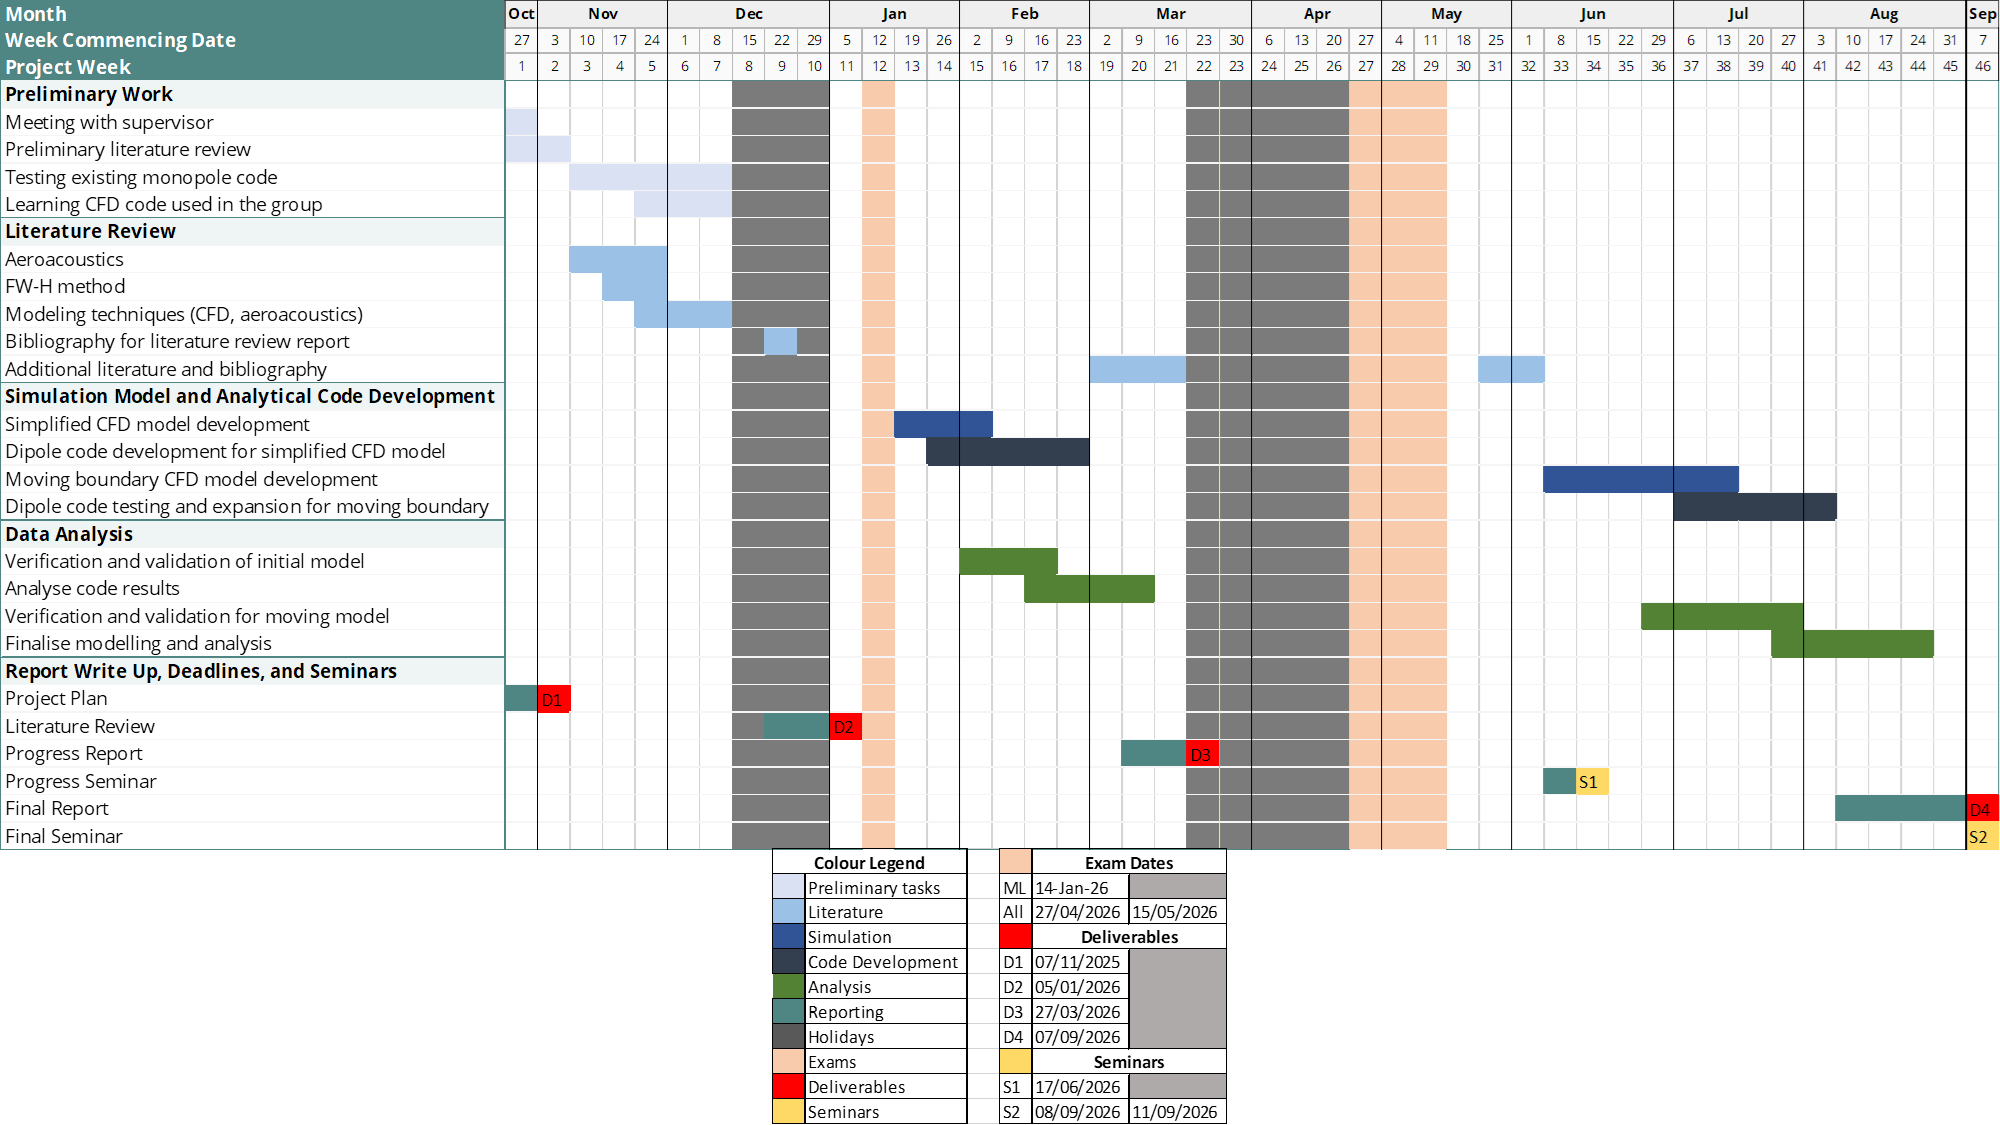
\includegraphics[width=1\linewidth]{fig_past_reports/gantt_chart.png}
    \caption{Gantt Chart of the research project}
    \label{fig:GC}
\end{figure}

\chapter{Variable Derivatives} \label{app:derivatives}

To derive the analytical point sources, a few definition for the derivatives are established.

\begin{equation}
    \left. \frac{\partial r}{\partial \tau} \right|_x =  -v_r
    \label{eq:C1}
\end{equation}

\begin{equation}
    \left. \frac{\partial M_r}{\partial \tau} \right|_x = \left( \frac{\partial M}{\partial \tau} \right)_r +
    \frac{c(M_r^2-|M|^2)}{r}
    \label{eq:C2}
\end{equation}

\begin{equation}
    \left. \frac{\partial |1-M_r|}{\partial\tau} \right|_x = \frac{(1-M_r)}{|1-M_r|}
    \left(
    -\left( \frac{\partial M}{\partial \tau}
    \right)_r  +
    \frac{c(|M|^2 - M_r^2}{r}
    \right)
    \label{eq:C3}
\end{equation}

\begin{equation}
    \left. \frac{\partial [Q(\tau)]_{\tau*}}{\partial\tau}\right|_x
    = \left.
    \left[ \frac{1}{1-M_r} \frac{\partial Q(\tau)}{\partial \tau} \right]_x
    \right|_{\tau*}
    \label{eq:C4}
\end{equation}

\begin{equation}
    \left. - \frac{\partial}{\partial x_i}
    \right|_t \int_S [Q_i]_{\tau*} dS =
    \left. \frac{\partial}{\partial t}\right|_x \int_S \left[ \frac{Q_ir_i}{cr}\right]_{\tau*}dS + \int_S \left[ \frac{Q_ir_i}{r^2}\right]_{\tau*}dS
    \label{eq:C5}
\end{equation}

% \chapter{Permeable Surface with Retarded Time Formulation} \label{app:fwh_expansion}

% Given the inhomogeneous wave equation in the integral form of the FW-H equation,
% \begin{equation}
%     \begin{split}
%         \Box^2p'(\bm{x},t) &=
%         \frac{\partial^2}{\partial x_i\partial x_j} \int_{-\infty}^{\infty} \frac{\overline{T_{ij}}\delta(g)J}{4\pi r}d^3\eta d\tau \\
%         &\quad - \frac{\partial}{\partial x_i} \int_{-\infty}^\infty \frac{\left(p_{ij}n_j+\rho u_i (u_n-v_n) \right) \delta(f)\delta(g) |\nabla_xf|J}{4\pi r} d^3\eta d\tau \\
%         &\quad + \frac{\partial}{\partial t} \int_{-\infty}^\infty \frac{\left(\rho_0u_n + \rho'(u_n-v_n) \right) \delta(f)\delta(g) |\nabla_xf|J}{4\pi r}d^3\eta d\tau
%     \end{split}
%     \label{eq:FWH}
% \end{equation}

% The first RHS term, the quadrupole, is not dealt with explicitly \cite{Parry1988, Hanson1985} as it is more significant for transonic and supersonic Mach numbers \cite{FfowcsWilliams1969, Ffowcs1969}. By choosing a sufficiently large permeable surface, the quadrupole contributions outside of this surface is negligible,

% \begin{equation}
%     \begin{split}
%         \Box^2p'(\bm{x},t) &=
%         - \frac{\partial}{\partial x_i} \int_{-\infty}^\infty \frac{\left(p_{ij}n_j+\rho u_i (u_n-v_n) \right) \delta(f)\delta(g) |\nabla_xf|J}{4\pi r} d^3\eta d\tau \\
%         &\quad + \frac{\partial}{\partial t} \int_{-\infty}^\infty \frac{\left(\rho_0u_n + \rho'(u_n-v_n) \right) \delta(f)\delta(g) |\nabla_xf|J}{4\pi r}d^3\eta d\tau
%     \end{split}
%     \label{eq:FWH_no_quad}
% \end{equation}

%  Using the notation by di Francescantonio \cite{Francescantonio1997} to simplify the algebra, new variables $U_i$ and $L_i$ are introduced to represent mass and momentum fluxes through the control surface,

% \begin{equation*}
%     U_i=(1-\frac{\rho}{\rho_0})v_i  + \frac{\rho}{\rho_0}u_i \quad     L_i=p_{ij}n_j+pu_i(u_n-v_n)
% \end{equation*}

% Considering an undistorted control surface that translates at a constant and subsonic velocity, the retarded time formulation, as described by Brentner and Farassat \cite{Brentner1998} is,

% \begin{equation}
% \begin{split}
%     p'(\bm{x}, t) &= \frac{1}{4\pi} \int_{S} \left[ \frac{\rho_0 (\dot{U}_n + U_{\hat{n}})}{r(1-M_r)^2} \right]_{\tau^*} dS(\eta) \\
%     &\quad + \frac{1}{4\pi} \int_{S} \left[ \frac{\rho_0 (r(dM/d\tau)_r + c(M_r - |M|^2))}{r^2(1-M_r)^3} \right]_{\tau^*} dS(\eta) \\
%     &\quad + \frac{1}{4\pi c} \int_{S} \left[ \frac{\dot{L}_r}{r(1-M_r)^2} \right]_{\tau^*} dS(\eta) \\
%     &\quad + \frac{1}{4\pi} \int_{S} \left[ \frac{L_r - L_m}{r^2(1-M_r)^2} \right]_{\tau^*} dS(\eta) \\
%     &\quad + \frac{1}{4\pi c} \int_{S} \left[ \frac{L_r(r(dM/d\tau)_r + c(M_r - |M|^2))}{r^2(1-M_r)^3} \right]_{\tau^*} dS(\eta)
% \end{split}
% \label{eq:fwh_full_expansion_ch2}
% \end{equation}

% The retarded time are calculated implicitly via the Newton-Raphson root-finding method. 

\chapter{Green's Function for Wave Equations} \label{app:GF}
Given a wave equation,
\begin{equation*}
    \left(\nabla^2 - \frac{1}{c^2}\frac{\partial^2}{\partial t^2} \right) \psi(\hat{r},t)=-f(\hat{r},t)
\end{equation*}

Green's function of the above equation,
\begin{equation*}
    \left(\nabla^2 - \frac{1}{c^2}\frac{\partial^2}{\partial t^2} \right) G(\hat{r},t |\hat{r'},t')=-\delta(\hat{r'}-\hat{r})\delta(t-t')
\end{equation*}

Let $\hat{r'}=0$ and $t'=0$. Solving for $\nabla^2G$
\begin{equation*}
    \begin{split}
        \nabla^2G(\hat{r},t) &= \frac{1}{r^2}\frac{\partial}{\partial r} \left(r^2 \frac{\partial}{\partial r} \right)G \\
        &\quad =\frac{1}{r} \frac{\partial G}{\partial r} + \frac{1}{r} \left( \frac{\partial G}{\partial r} + r \frac{\partial^2G}{\partial r^2} \right) \\
        &\quad = \frac{1}{r} \frac{\partial^2}{\partial r^2} (rG).
    \end{split}
\end{equation*}

Substituting back to the wave form,
\begin{equation*}
    \nabla^2G - \frac{1}{c^2}\frac{\partial^2}{\partial t^2}G=-\delta(r)\delta(t)
\end{equation*}
\begin{equation*}
    \frac{1}{r}\frac{\partial^2}{\partial r^2}(rG) - \frac{1}{c^2}\frac{1}{r}\frac{\partial^2}{\partial t^2} (rG)=-\delta(r)\delta(t)
\end{equation*}

Factoring the differential terms, it is found that if $r>0$, then the left-hand side term is equal to zero,

\begin{equation}
    \left[\left(\frac{1}{c}\frac{\partial}{\partial t} + \frac{\partial}{\partial r} \right)\left(\frac{1}{c}\frac{\partial}{\partial t} - \frac{\partial}{\partial r} \right) \right](rG)=0
    \label{eq:green_step1}
\end{equation}

Then, let $u=ct-r$ and $v=ct+r$, it will be found that,
\begin{equation*}
    \frac{\partial}{\partial u} = \frac{1}{2} \left(\frac{1}{c}\frac{\partial}{\partial t} -\frac{\partial}{\partial r}\right)
    \quad
    \frac{\partial}{\partial v} = \frac{1}{2} \left(\frac{1}{c}\frac{\partial}{\partial t} +\frac{\partial}{\partial r}\right)
\end{equation*}

Given that $\partial^2(rG)/(\partial u\partial v)=0$, if $rG=g(v)=g_+(ct+r)$ and $rG=g(u)=g_-(ct-r)$, then,

\begin{equation*}
    G=\frac{1}{r}g_{\pm}(ct\pm r)
\end{equation*}
\begin{equation*}
    G(\hat{r},t | \hat{r'},t')=\frac{1}{\hat{r}-\hat{r'}}g_{\pm}(c(t-t') \pm |\hat{r} - \hat{r'}|)
\end{equation*}

Taking $\nabla^2G$ using this definition,
\begin{equation*}
    \begin{split}
        \nabla^2G&=\nabla^2 \left(\frac{1}{r}g_{\pm}(ct\pm r) \right) =\nabla^2 \left(\frac{1}{r}\nabla g_{\pm} + g_{\pm} \nabla \left(\frac{1}{r} \right) \right) \\
        &\quad = - \frac{2}{r^2}\frac{\partial g}{\partial r} + \frac{2}{r^2}\frac{\partial g}{\partial r} + \frac{1}{r}\frac{\partial^2g}{\partial r^2} - 4\pi \delta(r)g
    \end{split}
\end{equation*}

The first two terms of the right-hand side cancel, and moving back to the wave equation format,

\begin{equation}
    \nabla^2G-\frac{1}{c^2}\frac{\partial^2}{\partial t^2}G = -\frac{1}{r} \left(\frac{1}{c^2}\frac{\partial^2}{\partial t^2} - \frac{\partial ^2}{\partial r^2}\right)g_{\pm} - 4\pi \delta(r)g_{\pm}
    \label{eq:green_step2}
\end{equation}

As described in equation \ref{eq:green_step1}, the first term of the right-hand side cancels. Going back to the wave equation,

\begin{equation*}
    \Box^2 \psi(\hat{r},t)=-\delta(\hat{r})\delta(t)=-4\pi \delta(\hat{r})g_{\pm}
\end{equation*}

Therefore, 
\begin{equation}
    \therefore \quad G_{\pm}=\frac{\delta(ct\pm r)}{4\pi r}
    \label{eq:greensfunction_derived}
\end{equation}

\chapter{Replacing \texorpdfstring{$\partial / \partial x_i$}/ Terms} \label{app:ddx_replace}

As the definition of dipoles are that of the spatial derivative of the forcing term convolved with the Green's function in 3D free-space, it is necessary to replace the spatial derivative terms to that of the temporal one to derive using the definitions described in Appendix \ref{app:derivatives}. As the goal is to transform $\textbf{x} \rightarrow \textbf{X}$ and $t\rightarrow\tau$, and the following are true: $\textbf{x}=\textbf{X}$ and $\tau=t-\frac{\textbf{r}}{c}$, then

\begin{equation*}
    \left. \frac{\partial}{\partial x_i} \right|_t = 
    \frac{\partial X_j}{\partial x_i} \frac{\partial}{\partial X_j} + \frac{\partial\tau}{\partial x_i} \frac{\partial}{\partial\tau}=\delta_{ij}\frac{\partial}{\partial X_j} - \frac{r_i}{cr(1-M_r)}\frac{\partial}{\partial\tau}
\end{equation*}

% As stated previously that $\textbf{x}=\textbf{X}$,

\begin{equation}
    \frac{\partial}{\partial x_i} = \frac{\partial}{\partial x_i} - \frac{r_i}{cr(1-M_r)}\frac{\partial}{\partial\tau}
\end{equation}

Similarly for the  time derivative,

\begin{equation*}
    \left. \frac{\partial}{\partial t} \right|_{\textbf{x}} = \frac{\partial X_j}{\partial t} \frac{\partial}{\partial X_j} + \frac{\partial\tau}{\partial t} \frac{\partial}{\partial \tau}
\end{equation*}

Assuming no mean flow, the first term of the right hand side, $\partial X_i/\partial t$ is equal to zero, leaving,

\begin{equation}
    \left. \frac{\partial}{\partial t} \right|_{\textbf{x}} = \frac{1}{1-M_r} \left. \frac{\partial}{\partial \tau} \right|_{\textbf{x}}
    \label{eq:retarded_time_def}
\end{equation}

\chapter{Monopole Velocity Derivations} \label{app:mono_u}
Using the momentum equation, assuming the flow has no mean flow and is inviscid, substituting the monopole definition into the pressure term, the second terms of both left- and right-hand are zero. Defining the pressure gradient by defining the pressure as monopole pressure definition,

\begin{equation*}
    - \frac{\partial p}{\partial x_i} =
    \frac{\partial}{\partial x_i} \frac{\partial}{\partial t} \left[
    \frac{Q(\tau)}{4\pi r (1-M_r)}
    \right]_{\tau*}
\end{equation*}

and cancelling the unsteady term from both sides gives the following for the momentum equation,

% \begin{equation*}
%     \rho_0 \frac{\partial u_i}{\partial t} =
%     \frac{\partial}{\partial x_i} \frac{\partial}{\partial t} \left[
%     \frac{Q(\tau)}{4\pi r (1-M_r)}
%     \right]_{\tau*}
% \end{equation*}

% cancelling the unsteady term from both sides leaves,

\begin{equation}
    u_i = \frac{1}{\rho_0} \frac{\partial}{\partial x_i} \left[ 
    \frac{Q(\tau)}{4\pi r (1-M_r)}
    \right]_{\tau *}
    \label{eq:monopole_spatial_derivative}
\end{equation}

Convolving with Green's function in free 3D-space is done to replace the spatial derivative into a temporal derivative,

\begin{equation*}
    p'(\bm{x}, t) = \frac{\partial}{\partial x_i} (Q_i \star G) =
    - \frac{\partial}{\partial t} \left( 
    Q_i \star \frac{x_iG}{c|\bm{x}|}
    \right) -
    Q_i \star \frac{x_i G}{|\bm{x}|^2}
    \label{eq:convolve_monopole}
\end{equation*}

which has the same form as the integral shown in Appendix \ref{app:derivatives}, Equation \ref{eq:C5}. Substituting the monopole source terms into $Q_i$, and converting to retarded time using the equation found in Appendix \ref{app:ddx_replace} Equation \ref{eq:retarded_time_def}, gives,

\begin{equation*}
    \frac{\partial}{\partial x_i} \left[ 
    \frac{Q(\tau)}{4\pi r (1-M_r)}
    \right]_{\tau*}
    = \frac{1}{1-M_r} \frac{\partial}{\partial\tau} \left[ 
    \frac{Q(\tau)r_i}{4\pi c \bm{r}^2 (1-M_r)^2}
    \right]_{\tau *}
    + \left[ 
    \frac{Q(\tau)r_i}{4 \pi r^3 (1-M_r)}
    \right]_{\tau*}
    \label{eq:monopole_velocity_underived}
\end{equation*}

which can then be solved analytically to give the solution for velocity,

\begin{equation}
    \begin{split}
    u_i 
    &= \frac{1}{4\pi\rho_0} \Bigg[ \frac{(\partial Q(\tau)/\partial \tau)r_i}{c r^2(1 - M_r)^2} 
    + \frac{Q(\tau)r_i}{r^3(1-M_r)^3}
    + \left(\frac{dM}{d\tau} \right) \frac{Q(\tau)r_i}{cr^2(1-M_r)^3} \\
    &\phantom{= \frac{1}{4\pi\rho_0}
    \Bigg[} - \frac{Q(\tau)M^2r_i}{r^3(1-M_r)^3}
    - \frac{Q(\tau)M_i}{r^2(1-M_r)^2}
    \Bigg]_{\tau*}
    \end{split}
    % \label{eq:monopole_velocity}
\end{equation}


\chapter{Dipole Velocity: Stationary Assumption} \label{app:zeroMach}
Defining pressure gradient from the momentum equation and dipole definition,

\begin{equation*}
    -\frac{\partial p}{\partial x_i} = 
    \frac{\partial^2}{\partial x_i \partial x_j} \left[ 
    \frac{f_i(\tau)}{4\pi r (1-M_r)}
    \right]_{\tau*}
\end{equation*}

Going back to momentum equation, the velocity is,

\begin{equation*}
    u_i = \frac{1}{4\pi\rho_0} \frac{\partial^2}{\partial x_i \partial x_j} \int_{-\infty}^t \frac{f_i(\tau)}{r(1-M_r)}dt
\end{equation*}

assuming $dr/dt=0$ and $M_r=0$, letting $F_i(\tau) = \int f_i(\tau) d\tau \implies f_i(\tau) = \dot{F}_i(\tau)$, and changing to integrating with respect to $\tau$, this simplifies the integrand to,

\begin{equation*}
    u_i = \frac{1}{4\pi r\rho_0} \frac{\partial^2}{\partial x_i \partial x_j} \int_{-\infty}^t {f_i(\tau)}d\tau
\end{equation*}

Taking the integral,

\begin{equation*}
    u_i = \frac{1}{4\pi r\rho_0} \frac{\partial^2}{\partial x_i \partial x_j} \int_{-\infty}^t {f_i(\tau)}d\tau
    =
    \frac{1}{4\pi r\rho_0} \frac{\partial^2}{\partial x_i \partial x_j} \left[F_i(\tau-r/c)
    \right]
\end{equation*}

Hence, the analytical solution for velocity that is valid for cases of zero relative Mach number between the source and observer for near- and far-field,

\begin{equation}
    u_i=\frac{1}{4\pi\rho_0} \left( 
    \frac{F_j(3n_in_j-\delta_{ij})}{r^3} +
    \frac{f_j(3n_in_j - \delta_{ij})}{cr^2} +
    \frac{\dot{f_j}(n_in_j)}{c^2r}
    \right)
    % \label{eq:dipole_u1}
\end{equation}

\chapter{Dipole Velocity: Plane Wave Assumption} \label{app:planeWave}

Given the plane wave,
\begin{equation}
    p'(\bm{x},t)=\frac{g(t-r/c)}{r}
    \label{eq:plane_wave_def}
\end{equation}

Taking the pressure gradient,

\begin{equation*}
    \frac{\partial p'}{\partial x_i} = 
    \left[\frac{\partial}{\partial x_i}\frac{1}{r}g \right] +
    \frac{1}{r} \left[ \frac{\partial}{\partial x_i}g 
    \right]
\end{equation*}

where the first and second terms correspond to the near- and far-field, respectively. The plane wave is valid only in the far-field, and taking the time derivative yields,

\begin{equation*}
    \frac{\partial p'}{\partial t} = \left[ 
    \frac{\partial}{\partial t} \frac{g}{r}
    \right]
    = \frac{1}{r} \frac{\partial}{\partial t} g(\tau) - g(\tau) \frac{v_r}{r^2}
\end{equation*}

In the far-field, $\frac{1}{r}\frac{\partial}{\partial t}g(\tau) \gg g(\tau) \frac{v_r}{r^2}$, simplifying the expression to,

\begin{equation*}
    \frac{\partial p'}{\partial t} \approx \frac{1}{r}\frac{\partial}{\partial t} g(\tau)
\end{equation*}

which gives the following expression,

\begin{equation*}
    \frac{\partial p'}{\partial x_i} = -\frac{n_i}{c} \frac{\partial p'}{\partial t}
\end{equation*}

substituting into the momentum equation provides the velocity equation for the plane wave,

\begin{equation}
    u_i = \frac{n_i}{\rho_0c}p'(\bm{x},t)
    % \label{eq:dipole_u2}
\end{equation}